\documentclass{beamer}

\usepackage{beamerthemesplit}
\usepackage{amsmath}
\usepackage{amsfonts}
\usepackage{amssymb}
\usepackage{qtree}
\usepackage{cancel}
\usepackage{tkz-graph}
%\usepackage[pdftex]{graphicx}

\makeatletter
\newcommand{\reallytiny}{\@setfontsize{\srcsize}{2pt}{2pt}}
\makeatother

\mode<presentation>
{
  \usetheme{metropolis}
  % or ...

  %\setbeamercovered{transparent}
  % or whatever (possibly just delete it)
}

\usepackage[english]{babel}
% or whatever

\usepackage[latin1]{inputenc}
% or whatever

\usepackage{times}
\usepackage[T1]{fontenc}

\title{Partial Operator Induction with Beta Distribution}

\author{Nil Geisweiller}

\institute[SingularityNET OpenCog Foundations] % (optional, but mostly needed)
{
  \begin{center}
    
\includegraphics[scale=0.35]{images/snet_oc_nmt.png}
  \end{center}
}

\date[AGI-18] % (optional, should be abbreviation of conference name)
{AGI-18\\
  Prague}

\AtBeginSection[]
{
  \begin{frame}<beamer>{Outline}
    \tableofcontents[currentsection,currentsection]
  \end{frame}
}

\AtBeginSubsection[]
{
  \begin{frame}<beamer>{Outline}
    \tableofcontents[currentsection,currentsubsection]
  \end{frame}
}

%\newcommand{\AND}{\textit{AND}}
%\newcommand{\OR}{\textit{OR}}
%\newcommand{\NOT}{\textit{NOT}}
\newcommand{\AND}{\land}
\newcommand{\OR}{\lor}
\newcommand{\NOT}{\lnot}

\begin{document}

\frame
{
  \maketitle
}
\section[Outline]{}
\frame{\tableofcontents}

\section{Problem:}
\subsection{Combining Models from Different Contexts}

\begin{frame}[fragile]
  \frametitle{Problem}

  How to combine models obtained from different contexts?

  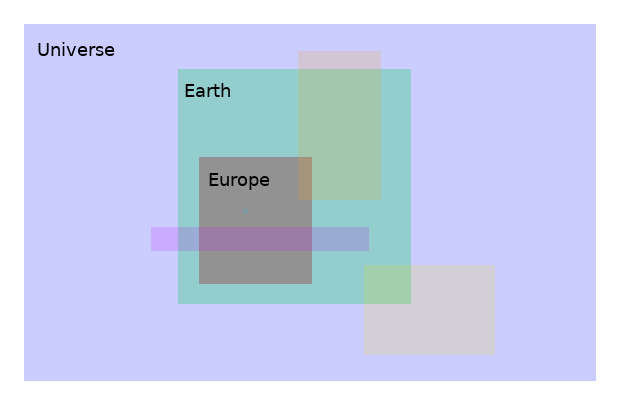
\includegraphics[scale=0.5]{images/Europe_Earth_Universe.png}
\end{frame}

% If you take the most specific model, with possibly the highest
% predictive power, you risk over-fitting. If you take the most general
% model, you risk under-fitting.

\begin{frame}[fragile]
  \frametitle{Solution}

  Bayesian Model Averaging (esp. Solomonoff Operator Induction)

  + partial models (obtained from different data sets)

  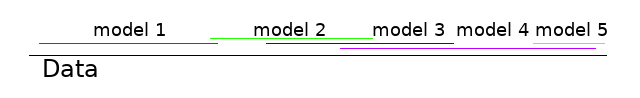
\includegraphics[scale=0.5]{images/data_line.png}
\end{frame}

\begin{frame}[fragile]
  \frametitle{Preserve Uncertainty}

  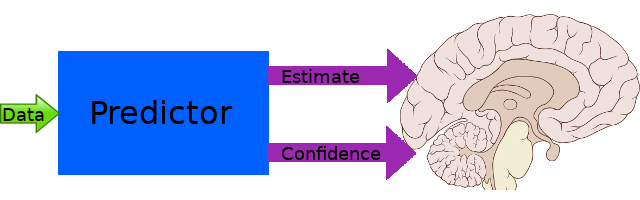
\includegraphics[scale=0.5]{images/preserve_uncertainty.png}
\end{frame}

\begin{frame}[fragile]
  \frametitle{Preserve Uncertainty}

  Exploration vs Exploitation (Thompson Sampling)

  \begin{center}
    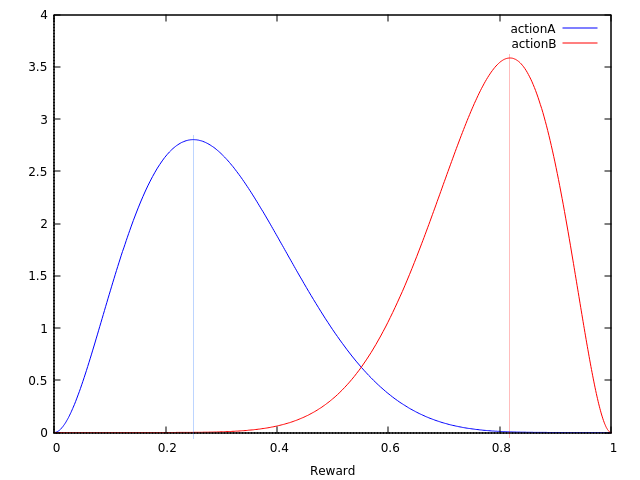
\includegraphics[scale=0.55]{images/ActionA_ActionB_lines_alpha.png}
  \end{center}
\end{frame}

\section{Theory:}
\subsection{Solomonoff Operator Induction and Beta Distribution}

\begin{frame}
  \frametitle{Solomonoff Operator Induction}

  Probability Estimate:
  $$
  \hat{P}(A_{n+1}|Q_{n+1}) = \sum_j a_0^j \prod_{i=1}^{n+1} O^j(A_i|Q_i)
  $$
  where:
  \begin{itemize}
  \item $Q_i$ = $i^{th}$ question
  \item $A_i$ = $i^{th}$ answer
  \item $O^j$ = $j^{th}$ operator
  \item $a^j_0$ = prior of $j^{th}$ operator
  \end{itemize}
\end{frame}

\begin{frame}
  \frametitle{Beta Distribution}

\begin{columns}

\column{2in}
  
  Probability Density Function:
  $$
    pdf_{\alpha, \beta}(x) = \frac{x^{\alpha - 1} (1-x)^{\beta - 1}}
    {B(\alpha, \beta)}
  $$

  Beta Function:
  $$
  B_x(\alpha, \beta) = \int_0^x p^{\alpha - 1}(1-p)^{\beta - 1} dp
  $$
  $$
  B(\alpha, \beta) = B_1(\alpha, \beta)
  $$

  \alert{Conjugate Prior:}
  $$
  pdf_{m+\alpha, n-m+\beta}(x)
  \propto
  x^m (1-x)^{n-m} pdf_{\alpha, \beta}(x)
  $$
  
\column{2in}
  
  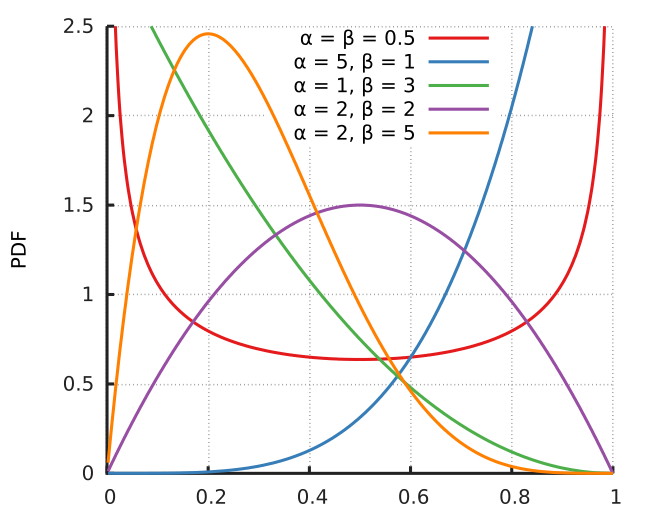
\includegraphics[scale=0.2]{images/Beta_distributions.png}

\end{columns}


% \begin{columns}
% \column{3in}
%   $$
%   pdf_{m+\alpha, n+\beta}(x)
%   \propto
%   x^m (1-x)^n pdf_{\alpha, \beta}(x)
%   $$
% \column{0.5in}
%   $$\Rightarrow$$
% \column{1in}
%   \begin{center}\textcolor{red}{Conjugate Prior}\end{center}
% \end{columns}

% \begin{beamerboxesrounded}{\textcolor{red}{Conjugate Prior}}
%   $$
%   pdf_{m+\alpha, n+\beta}(x)
%   \propto
%   x^m (1-x)^n pdf_{\alpha, \beta}(x)
%   $$
% \end{beamerboxesrounded}


\end{frame}

\begin{frame}[fragile]
  \frametitle{Beta Distribution Operator}

OpenCog implication link
{\small
\begin{verbatim}
  ImplicationLink <TV>
    R
    S
\end{verbatim}
}

$$
\equiv
$$

Class of parameterized operators

  $$
  O^j_p(A_i|Q_i) = \text{if}\ R^j(Q_i)\ \text{then}\
  \begin{cases}
    p, & \text{if}\ A_i = A_{n+1}\\
    1-p, & \text{otherwise}
  \end{cases}
  $$
\end{frame}

\begin{frame}
  \frametitle{Second Order Solomonoff Operator Induction}

  % \begin{columns}
  % \column{3in}
  
  Probability Estimate:
  $$
  \hat{P}(A_{n+1}|Q_{n+1}) = \sum_j a_0^j \prod_{i=1}^{n+1} O^j(A_i|Q_i)
  $$

  % $$
  % \Downarrow
  % $$
  
  Probability Distribution Estimate:
  $$
    \hat{cdf}_{(A_{n+1}|Q_{n+1})}(x) = \sum_{O^j(A_{n+1}|Q_{n+1}) \le x}
    a_0^j \prod_{i=1}^{n} O^j(A_i|Q_i)
  $$

  % \column{1in}

  % gotten from maxima:
  % plot2d([[discrete, [[0.67, 0.0]]], cdf_beta(x, 10.0, 5.0)], [x, 0,
  % 1], [style, points, lines], [point_type, asterisk], [legend, "P",
  % "cdf"]); plot2d([[discrete, [[0.67, 0.0]]], cdf_beta(x,

  \begin{center}
    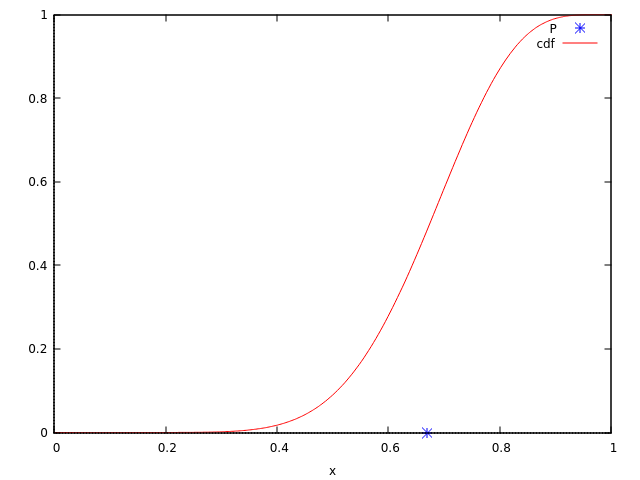
\includegraphics[scale=0.28]{images/P_vs_CDF_alpha.png}
  \end{center}

  % \end{columns}

\end{frame}

\begin{frame}
  \frametitle{Program Completion}
  $$
  \begin{array}{@{}ll@{}}
    O^j_{p, C}(A_i|Q_i) = &
                            \text{if}\ R^j(Q_i)\ \text{then}\
                            \begin{cases}
                              p, & \text{if}\ A_i = A_{n+1} \\
                              1-p, & \text{otherwise}
                            \end{cases}\\
                          & \text{else}\ C(A_i|Q_i)
  \end{array}
  $$
  % A \emph{completion} $C$ of $O^j_p$ is a program that completes
  % $O^j_p$ for the unaccounted data, when $R^j(Q_i)$ is false, such
  % that the operator once completed is as follows

  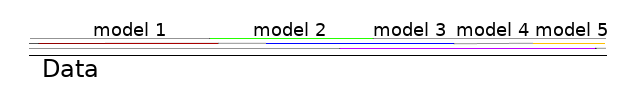
\includegraphics[scale=0.5]{images/data_line_completion.png}

\end{frame}

\begin{frame}
  \frametitle{Combing Solomonoff Operator Induction and\\
    Beta Distributions}

  $$
    \hat{cdf}_{(A_{n+1}|Q_{n+1})}(x) \propto \sum_j a_0^j r^j
    B_x(m^j+\alpha, n^j-m^j+\beta)
    B(m^j+\alpha, n^j-m^j+\beta)
  $$

  where
  \begin{itemize}
  \item $n^j$ = number of observations explained by $j^{th}$ model    
  \item $m^j$ = number of true observations explained by $j^{th}$ model
  \item $r^j$ = likelihood of the unexplained data
  \end{itemize}

  $r^j = ???$ \pause $\approx 2^{-v^{(1-c)}}$
  \begin{itemize}
  \item $v = n-n^j$ = number of unexplained observations
  \item $c$ = compressability parameter
    \begin{itemize}
    \item $c=1$ $\rightarrow$ explains remaining data% (down to one
      %bit)
    \item $c=0$ $\rightarrow$ can't explain remaining data
    \end{itemize}
  \end{itemize}
\end{frame}

\section{Practice:}
\subsection{Inference Control Meta-Learning}

\begin{frame}[fragile]
  \frametitle{Inference Control Meta-learning}
  \begin{center}\textcolor{blue}{Learn how to reason efficiently}\end{center}

  Methodology:
  \begin{enumerate}
  \item<+-> Solve sequence of problems (via reasoning)
  \item<+-> Store inference traces
  \item<+-> Mine traces to discover patterns
  \item<+-> Build control rules
{\small
\begin{semiverbatim}
  Implication <TV>
    And
      \textcolor{blue}{<inference-pattern>}
      \textcolor{red}{<rule>}
    \textcolor{green}{<good-inference>}
\end{semiverbatim}
}  
  \item<+-> \textcolor{red}{Combine control rules to guide future
      reasoning}
    % \begin{itemize}
    % \item Efficient
    % \item Accurate
    % \end{itemize}
  \end{enumerate}
\end{frame}

\begin{frame}[fragile]
  \frametitle{Combine Control Rules}

\begin{columns}

\column{1.1in}

{\tiny
\begin{semiverbatim}
Implication <TV1>
  And
    \textcolor{blue}{<inference-pattern-1>}
    \textcolor{red}{deduction-rule}
  \textcolor{green}{<good-inference>}
\end{semiverbatim}
}

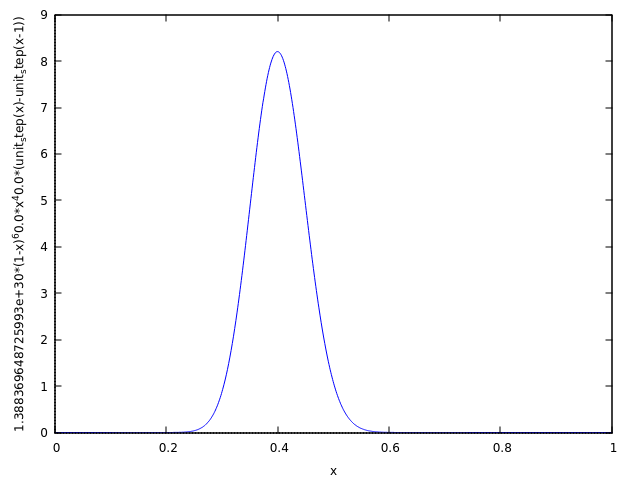
\includegraphics[scale=0.2]{images/Beta_40_60_alpha.png}

\column{0.4in}
\begin{center}
  $$\oplus$$
  {\tiny $$c=0.01$$}
\end{center}

\column{1.3in}

{\tiny
\begin{semiverbatim}
Implication <TV2>
  And
    \textcolor{blue}{<inference-pattern-2>}
    \textcolor{red}{deduction-rule}
  \textcolor{green}{<good-inference>}
\end{semiverbatim}
}

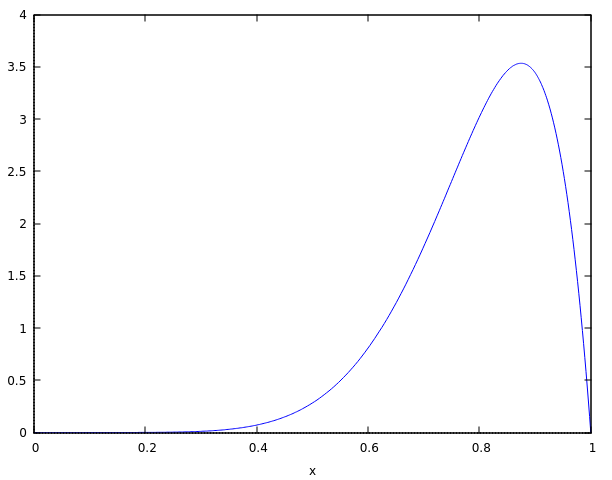
\includegraphics[scale=0.2]{images/Beta_8_2_alpha.png}

\end{columns}

$$=$$

\begin{center}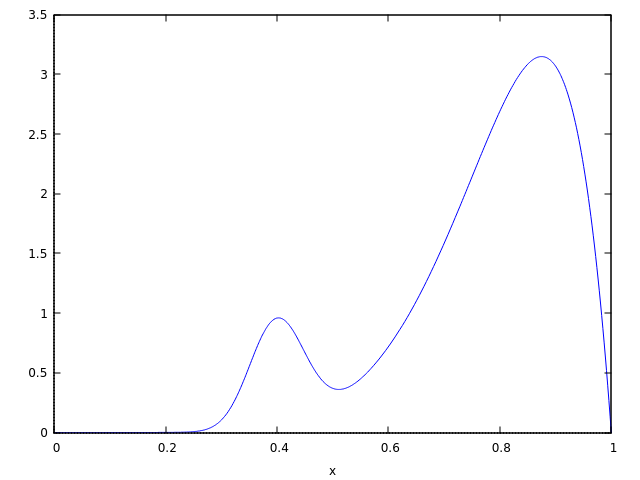
\includegraphics[scale=0.2]{images/Beta_mixed_c_0_01_alpha.png}\end{center}

\end{frame}

% \begin{frame}
%   Thanks you
% \end{frame}

% What this little bump does is that when this distributed is handed
% to the decision process it'll be able to sample the probability of
% success of that action in a more nuanced way, and hopefully have a
% better balance between exploration and exploitation.

\begin{frame}
  \frametitle{Conclusion}

  Contribution:
  \begin{itemize}
  \item Second Order Solomonoff Operator Induction
  \item Specialized for Beta Distribution
  \item Attempt to Deal with Partial Models
  \end{itemize}

  \pause
  
  Future Work:
  \begin{itemize}
  \item Improve Likelihood of Unaccounted Observations
  \item More Experiments (Inference Control Meta-learning)
  \end{itemize}

  \pause

  \begin{center}
    Thank you!
  \end{center}

\end{frame}

\end{document}
